\documentclass[12pt, a4paper]{report}

% ========== PACKAGES UTILES ==========
\usepackage[utf8]{inputenc}
\usepackage[T1]{fontenc}
\usepackage[french]{babel}
\usepackage{amsmath, amssymb}
\usepackage{graphicx}
\usepackage{geometry}
\usepackage{xurl}
\usepackage{titlesec}
\usepackage{fancyhdr}
\usepackage{hyperref}
\usepackage{xcolor}
\usepackage{booktabs}
\usepackage{listings}
\usepackage{enumitem}
\usepackage{ragged2e}
\usepackage{abstract}
\usepackage{tcolorbox}
\usepackage{caption}
\usepackage{subcaption}
\usepackage{float}

% ========== MISE EN PAGE ==========
\geometry{left=2.5cm, right=2.5cm, top=2.5cm, bottom=2.5cm}
\setlength{\parindent}{0pt}
\setlength{\parskip}{0.5em}
\linespread{1}

% ========== COULEURS ==========
\definecolor{noir}{RGB}{0,0,0}
\definecolor{gris}{RGB}{100, 100, 100}

\setlist[itemize]{label=\textbullet, noitemsep, topsep=0.3em}

% ============================================================
% EN-TÊTE ET PIED DE PAGE
% ============================================================
\pagestyle{fancy}

\fancyhead{}
\fancyhead[L]{\small\textsc{Prédiction des accidents maritimes}}
\fancyhead[R]{\small\textsc{Université de la Nouvelle-Calédonie}}
\renewcommand{\headrulewidth}{0.4pt}

\fancyfoot[C]{\small Axel Archambeault \& Ashley Roo --- \thepage}
\renewcommand{\footrulewidth}{0.5pt}

% Style plain normal
% Utilisé notamment par les premières pages des chapitres
\fancypagestyle{plain}{
  \fancyhead{}
  \fancyhead[L]{\small\textsc{Prédiction des accidents maritimes}}
  \fancyhead[R]{\small\textsc{Université de la Nouvelle-Calédonie}}
  \fancyfoot[C]{\small Axel Archambeault \& Ashley Roo --- \thepage}
  \renewcommand{\headrulewidth}{0.4pt}
  \renewcommand{\footrulewidth}{0.5pt}
}

% Style vide
% Utilisé pour les pages sans numéro
\fancypagestyle{vide}{
  \fancyhead{}
  \fancyfoot{}
  \renewcommand{\headrulewidth}{0pt}
  \renewcommand{\footrulewidth}{0pt}
}

% ========== TITRES ==========
\titleformat{\chapter}
  {\normalfont\LARGE\bfseries}{\thechapter}{1em}{}

\titleformat{\section}
  {\normalfont\Large\bfseries}{\thesection}{1em}{}

\titleformat{\subsection}
  {\normalfont\large\bfseries}{\thesubsection}{1em}{}

\titlespacing*{\chapter}{0pt}{-1.5em}{0.5em}
\titlespacing*{\section}{0pt}{0.5em}{0.3em}
\titlespacing*{\subsection}{0pt}{0.3em}{0.2em}

% ========== HYPERLIENS ==========
\hypersetup{
  colorlinks=true,
  linkcolor=black,
  urlcolor=black,
  citecolor=black
}

% ========== DOCUMENT ==========
\begin{document}

% ============================================================
% PAGE DE GARDE
% ============================================================
\begin{titlepage}
  \thispagestyle{empty}
  \centering

  \vspace*{1cm}
  \IfFileExists{UNC.jpg}{
\includegraphics[width=0.25\textwidth]{UNC.jpg}}{\fbox{\parbox[c][3cm][c]{0.25\textwidth}{\centering Logo indisponible}}} \\[1cm]


  {\Huge \textbf{Prédiction des accidents maritimes}} \\[0.5cm]

  \textbf{Auteurs :} \\
  Axel Archambeault \\
  Ashley Roo \\[1cm]

  \textbf{Tuteur :} \\
  M. Salmon \\
  Mme. Selmaoui \\[1cm]

  \vfill

  \textit{Licence informatique TREC 5}\\
  \textit{2026}

  \vspace*{1cm}

\end{titlepage}

% ============================================================
% RÉSUMÉ (sans en-tête ni pied de page)
% ============================================================
\chapter*{Résumé}
\thispagestyle{empty}
\addcontentsline{toc}{chapter}{Résumé}

text

\clearpage

% ============================================================
% TABLE DES MATIÈRES (sans en-tête ni pied de page)
% ============================================================
\pagestyle{empty}

{% groupe local : le style "plain" est neutralisé le temps du \tableofcontents
  \fancypagestyle{plain}{
    \fancyhf{}
    \renewcommand{\headrulewidth}{0pt}
    \renewcommand{\footrulewidth}{0pt}
  }
  \tableofcontents
}

\clearpage

% ============================================================
% DÉBUT DU RAPPORT
% ============================================================
\pagestyle{fancy}
\pagenumbering{arabic}
\setcounter{page}{1}


% ============================================================
% DÉBUT DU RAPPORT
% ============================================================
% La numérotation commence ici à 1
\pagestyle{fancy}
\pagenumbering{arabic}
\setcounter{page}{1}


% ============================================================
% CHAPITRE 1 : INTRODUCTION
% ============================================================
\chapter{Introduction}
\thispagestyle{plain}

\section{Contexte}

Depuis la nuit des temps, l'être humain a navigué de nombreuses contrées, on peut citer la découverte de l'Amérique en 1492 par Christophe Colomb, qui a révolutionné notre manière de naviguer. Cependant, les activités maritimes ne sont pas sans risques comme l'illustre notamment le naufrage du Titanic réputé insubmersible. De nos jours, le transport maritime représente environ 80~\% du commerce mondial en volume, et les accidents ne sont pas sans conséquences notamment des conséquences économiques et plus rares humaines.

\section{Problématique et objectifs}

C'est dans ce contexte que s'insère notre projet tutoré dont l'objectif principal est de mettre en avant les zones à risques, de comprendre les facteurs associés aux accidents maritimes et d'anticiper leurs évolutions grâce à des modèles de prédiction. Nous nous demanderons donc comment identifier ces zones à risques mais aussi comment anticiper les accidents en mer à l'aide d'outils de prédiction afin de contribuer à la sécurité maritime et à la prévention des risques.

\section{Cadre du projet}

\subsection{Méthodologie et technique}

C'est pour cela que nous nous sommes appuyés sur différents outils. Tout d'abord l'analyse de données, nous a permis de traiter et d'exploiter les informations obtenues. Ensuite les graphiques ainsi que les cartes interactives nous ont servi à visualiser ces données de manière claire et à identifier les zones et les tendances significatives. La programmation en Python nous a permis de mettre en oeuvre les différentes étapes du traitement et de développer les modèles de prédiction.

\subsection{Institutionnel}

Ce projet est réalisé dans le cadre de la licence informatique, en partenariat avec l'ISEA et les encadrants Monsieur Salmon et Madame Selmaoui. Il répond à une mission portant sur l'analyse et la prédiction des risques maritimes.

\subsection{Thématique}

Notre étude repose sur trois notions indispensables : la sécurité maritime, les risques et accidents en mer et pour finir la prédiction venant de modèles adaptés.

\subsection{Spatial}

Bien que les données d'accidents couvrent le monde entier, notre étude se restreint à l'Europe, ce choix s'explique par une disponibilité plus importante des données dans cette zone, ainsi qu'un besoin de cohérence avec des données de densité du trafic maritime. Pour notre étude, la zone est divisée en cellules.

\subsection{Temporel}

L'étude porte sur les accidents maritimes survenus entre le 17 juin 2011 et le 30 novembre 2025. Cependant les données de densité de trafic maritime couvrent la période entre 2017 à 2021.


% ============================================================
% CHAPITRE 2 : REVUE DE LITTÉRATURE
% ============================================================
\chapter{Revue de littérature}

\section{Prédiction des risques maritimes}

\section{Apports de la littérature sur la piraterie maritime}

\section{Méthodes prédictives}

\section{Positionnement de notre travail}


% ============================================================
% CHAPITRE 3 : DONNÉES ET PRÉTRAITEMENT
% ============================================================
\chapter{Données et prétraitement}

\section{Description des données}

Ce projet repose sur trois jeux de données distincts : les accidents maritimes, la flotte globale et la densité de trafic maritime. Ils apportent des renseignements complémentaires sur les accidents, le trafic maritime et le contexte dans lequel ils se produisent. Les trois sont fournis au format CSV.

\textbf{Accidents maritimes.} Le premier jeu de données recense les accidents maritimes survenus entre le 17 juin 2011 et le 30 novembre 2025, soit environ 44~000 enregistrements. Chaque ligne décrit un accident avec de nombreuses caractéristiques : la date et l'heure, la zone maritime, les coordonnées (latitude et longitude), la gravité de l'événement, le type de navire impliqué, la nature de l'accident ainsi que les dommages humains et matériels associés. Cette richesse de variables permet de faire une analyse exploratoire. Les données proviennent de la plateforme European Marine Casualty Information Platform (EMCIP), mise à disposition par l'European Maritime Safety Agency (EMSA). Ces données couvrent le monde entier, nous avons choisi de restreindre notre étude à l'Europe, pour des raisons expliquées dans la section suivante.

La distinction entre type d'accident et cause humaine reflète la structure de la base EMCIP : le type d'accident décrit l'événement observé (une collision, un contact, un échouement), tandis que la cause humaine permet de caractériser certains facteurs humains associés à l'événement (perte de contrôle, erreur de veille).

\textbf{Densité de trafic maritime (AIS).} Notre second jeu de données, issu de Vessel Density, est fourni par Cogea et accessible via la plateforme EMODnet ERDDAP. Ces données permettent de caractériser la densité du trafic maritime sur différentes zones géographiques, uniquement sur l'Europe. Elles nous fournissent une mesure de la densité de trafic, les données couvrent la période 2017-2021 et sont organisées mensuellement. Chaque enregistrement contient une date, des coordonnées et une valeur de densité.

\textbf{Flotte mondiale.} Le dernier jeu de données en notre possession décrit l'évolution de la flotte mondiale sur la période 2011-2026. Il est structuré par année, par type de navire (flotte totale, pétroliers, vraquiers, navires de charge classique, porte-conteneurs et autres navires) et par pavillon. Toutefois, dans le cadre de ce projet, il n'a été que très marginalement exploité : nous l'avons conservé comme variable de contexte, mais il n'a pas été intégré de manière significative.

\section{Préparation et nettoyage}

Avant d'utiliser les données pour l'analyse et la modélisation, un nettoyage et un prétraitement ont été réalisés afin de les rendre exploitables.

Pour les données d'accidents, les doublons et les données inutilisables ont été supprimés. Les coordonnées géographiques, initialement fournies sous un autre format, ont été converties en degrés décimaux afin de faciliter leur utilisation pour l'analyse spatiale. Par exemple, une position peut être représentée sous la forme \texttt{-4.617..., 53.320...}.

Plusieurs variables ont ensuite été ajoutées afin de faciliter l'analyse. À partir des informations temporelles et géographiques, nous avons notamment créé les variables \texttt{annee}, \texttt{saison} et \texttt{heure}, ainsi que \texttt{lat} et \texttt{long} pour la localisation des accidents. D'autres variables ont également été ajoutées pour caractériser les accidents : \texttt{gravite}, \texttt{port}, \texttt{bateau}, \texttt{type\_accident} et \texttt{cause\_accident\_humain}.

La précision des coordonnées restant limitée pour certains accidents, quelques points peuvent apparaître légèrement décalés sur les cartes, notamment avec certains points situés sur des zones terrestres. Ces imprécisions doivent donc être prises en compte lors de l'interprétation des cartes.

Les données de Vessel Density ont également été transformées. Initialement, elles étaient fournies sous la forme de coordonnées x et y, accompagnées de la date et de la valeur de densité (vd). Ces coordonnées ont été converties en variables latitude et longitude, afin d'obtenir une structure plus facilement exploitable et de permettre la mise en relation des données de trafic avec les accidents.

Après ces différentes étapes, les données obtenues ont pu être utilisées pour l'analyse spatiale et temporelle, notamment pour leur association aux différentes cellules géographiques.

\section{Construction du maillage}

Afin de réaliser l'analyse spatiale, nous avons divisé la zone étudiée en une grille composée de cellules de 1,5° de latitude × 1,5° de longitude. Seules les cellules correspondant aux zones couvertes par les données de densité de trafic maritime ont été conservées, soit 1~495 cellules.

Les coordonnées des accidents sont ensuite converties en coordonnées métriques (EPSG:3035). Chaque accident est associé au point de densité maritime le plus proche, avec une distance maximale de 50~km. Les accidents sont ainsi reliés à la grille utilisée pour les données de trafic.

La création de la grille et l'association des accidents aux points de densité maritime ont été réalisées avec les bibliothèques NumPy, utilisée notamment pour les opérations numériques, et pandas, utilisée pour la gestion et la manipulation des données, notamment des fichiers CSV.

\section{Agrégation spatio-temporelle}

\section{Processus global de traitement}


% ============================================================
% CHAPITRE 4 : ANALYSE EXPLORATOIRE
% ============================================================
\chapter{Analyse exploratoire et sélection des variables}

\section{Évolution des accidents dans le temps}

Cette première étape vise à étudier l'évolution du nombre d'accidents au cours du temps. La figure~\ref{fig:evolution_temporelle} représente le nombre d'accidents enregistrés chaque année entre 2011 et 2025 sur la zone de l'Europe.

\begin{figure}[H]
    \centering
    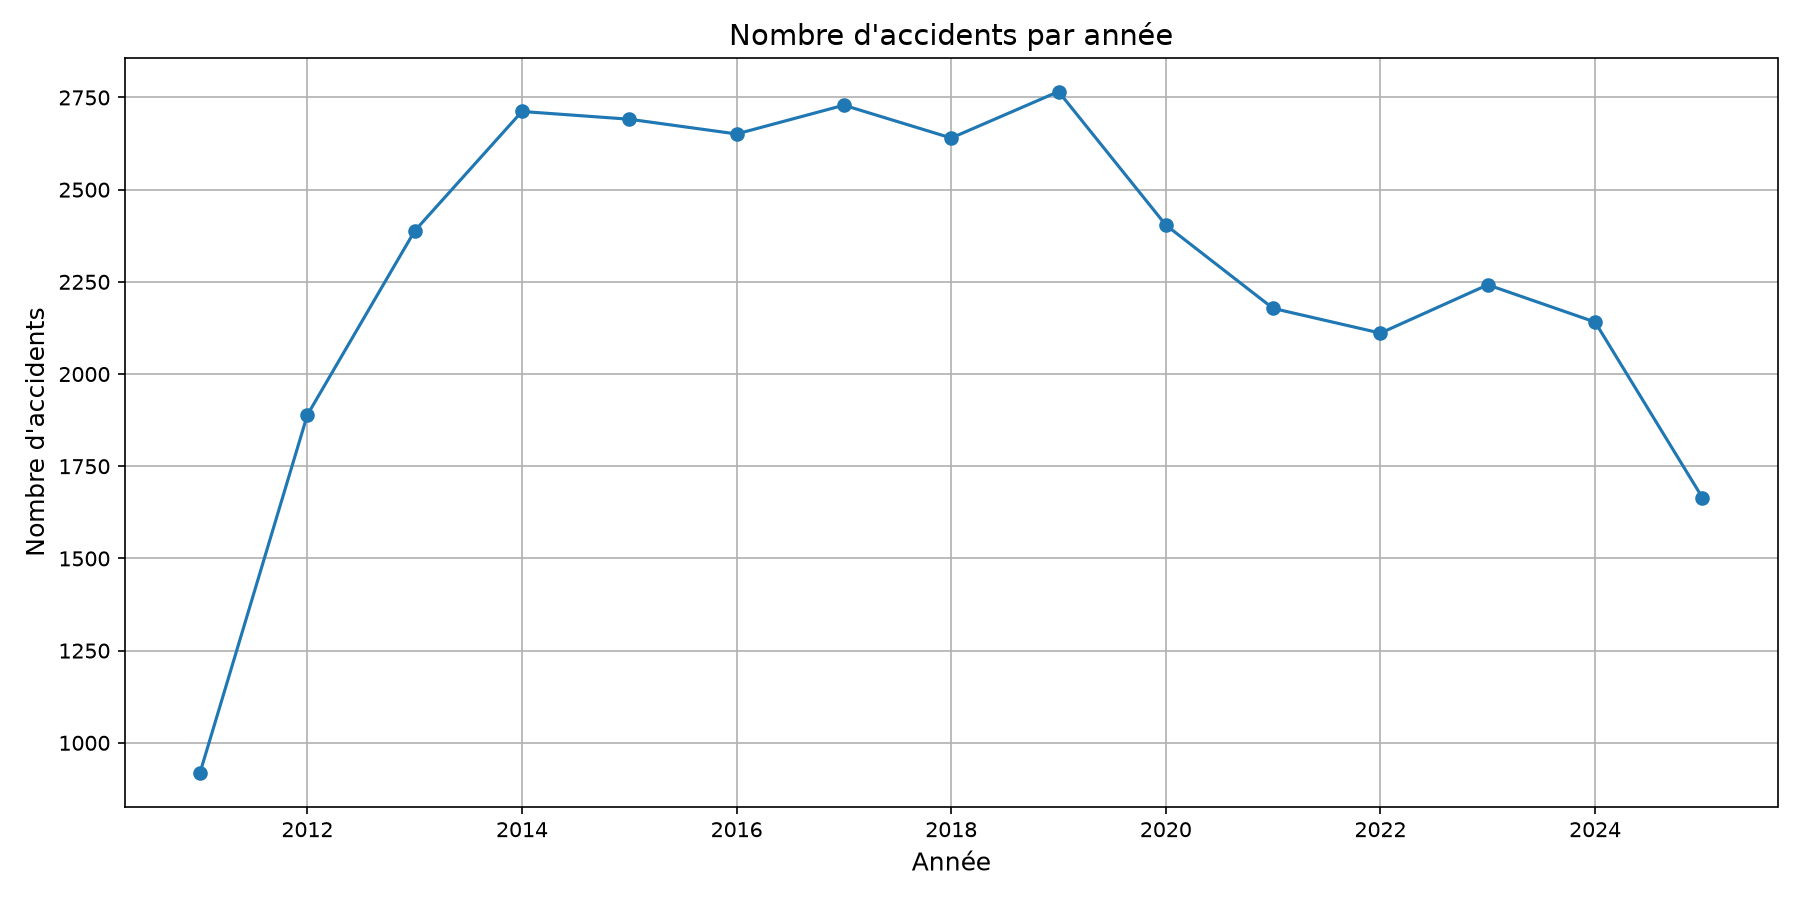
\includegraphics[width=0.9\textwidth]{graph_accident_by_years_eu.png}
    \caption{Évolution du nombre d'accidents maritimes en Europe (2011-2025).}
    \label{fig:evolution_temporelle}
\end{figure}

On peut constater une forte augmentation entre 2011 et 2013. Cette évolution s'explique par la mise en place progressive du système EMCIP et l'amélioration du signalement des accidents par les États membres. L'EMSA estimait alors qu'il y avait encore environ 30~\% de sous-déclaration en 2013, principalement à cause de la mise en place progressive du système EMCIP. Tout cela est lié à la mise en place de la directive européenne 2009/18/CE : depuis le 17 juin, les États membres doivent notifier certains accidents maritimes dans EMCIP, mais son application n'a pas été immédiate dans tous les États membres.

Entre 2014 et 2019, le nombre d'accidents reste relativement stable, autour de 2~600 et 2~750 par an. On peut noter une baisse importante de 2~750 en 2019 à 2~400 environ pour 2020. Cette forte diminution s'explique par la crise de la COVID-19, qui a entraîné une baisse du trafic maritime européen. Après 2020, le nombre d'accidents reste globalement inférieur au niveau observé avant la crise.

\section{Répartition géographique des accidents}

La répartition géographique des accidents montre une forte concentration dans certaines zones maritimes. Les principales concentrations sont observées dans la mer du Nord, notamment autour des grands ports d'Europe du Nord, ainsi que dans la Manche et le détroit du Pas-de-Calais. D'autres concentrations apparaissent autour de la Grèce, dans la Méditerranée occidentale et au niveau du détroit de Gibraltar. On constate aussi que les zones éloignées des ports et principaux axes maritimes présentent généralement moins d'accidents.

\begin{figure}[H]
    \centering
    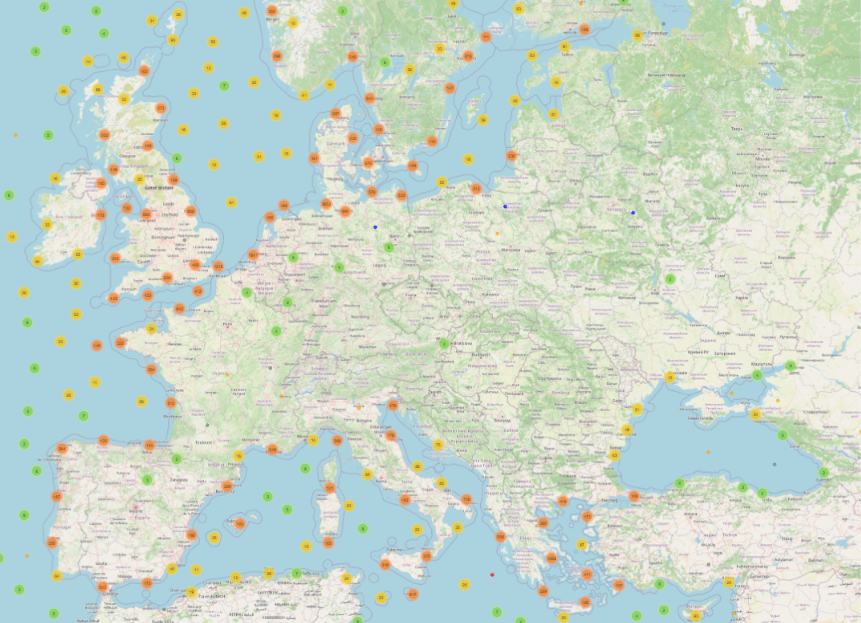
\includegraphics[width=0.9\textwidth]{carte_eu.png}
    \caption{Répartition géographique des accidents maritimes en Europe.}
    \label{fig:carte_accidents}
\end{figure}

Cette répartition peut être rapprochée de certains grands espaces économiques et axes de circulation européens. La Blue Banana, ou dorsale européenne, correspond historiquement à un espace fortement concentré en activités économiques et urbaines, allant approximativement du sud du Royaume-Uni jusqu'au nord de l'Italie. Le rapport du Parlement européen souligne également l'importance de cet espace pour les activités logistiques et portuaires européennes.

Plus au nord, la concentration observée autour de la mer du Nord, du Danemark et du sud de la Scandinavie peut davantage être rapprochée de l'axe STRING, qui relie notamment Hambourg aux principales régions de Scandinavie. Ces deux concepts permettent ainsi de replacer les concentrations observées sur notre carte dans le contexte des grands espaces économiques et des axes de transport européens. Il faudra cependant comparer ces observations avec la Vessel Density afin de déterminer si ces concentrations sont également associées à une forte densité de trafic maritime.

\section{Analyse des caractéristiques des accidents}

Après avoir étudié l'évolution temporelle et la distribution spatiale des accidents, nous allons nous intéresser aux caractéristiques propres aux accidents telles que leur gravité, leur nature, leurs causes, ainsi que l'influence de facteurs externes comme les saisons ou le type de navire impliqué.


\begin{figure}[H]
  \centering
  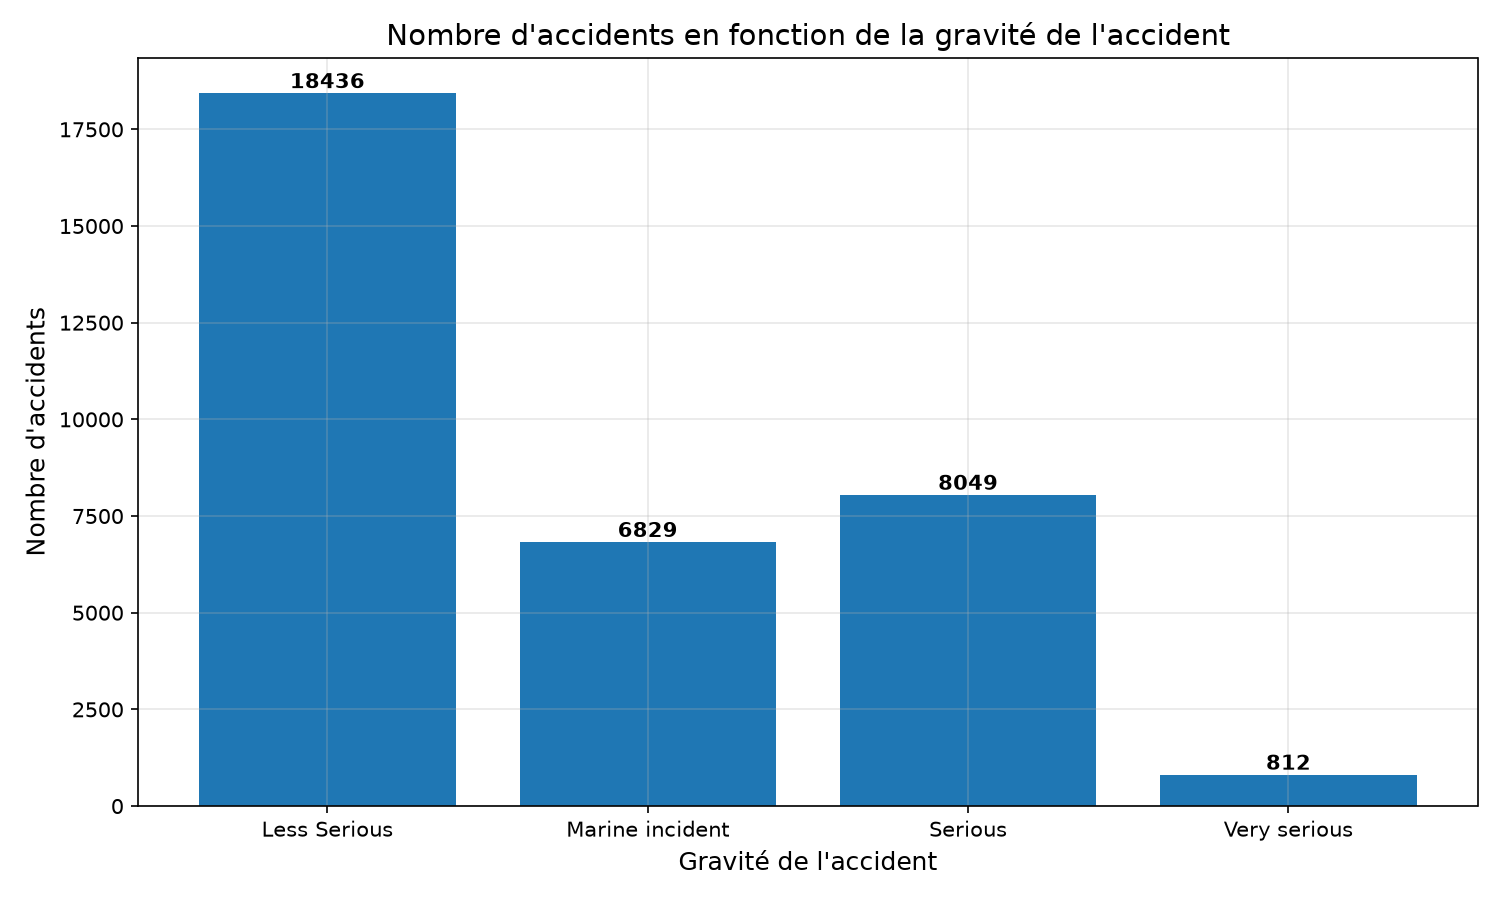
\includegraphics[width=0.8\textwidth]{graph_accident_by_severity_europe.png}
  \caption{Répartition des accidents selon leur gravité.}
  \label{fig:gravite}
\end{figure}
\textbf{Gravité.} La figure~\ref{fig:gravite} montre la répartition des accidents selon leur gravité. On observe une prédominance des accidents \og Less Serious \fg{} ($\sim$54~\%) suivis des accidents \og Serious \fg{} ($\sim$23,6~\%) et des \og Marine incident \fg{} ($\sim$20~\%) c'est un événement moins grave qu'un accident maritime, qui aurait pu conduire à un accident maritime, ou qui a entraîné des dommages mineurs et les \og Very serious \fg{} sont très minoritaires ($\sim$2,4~\%), ce qui montre que les accidents les plus graves représentent une faible proportion des événements enregistrés.


\begin{figure}[H]
  \centering
  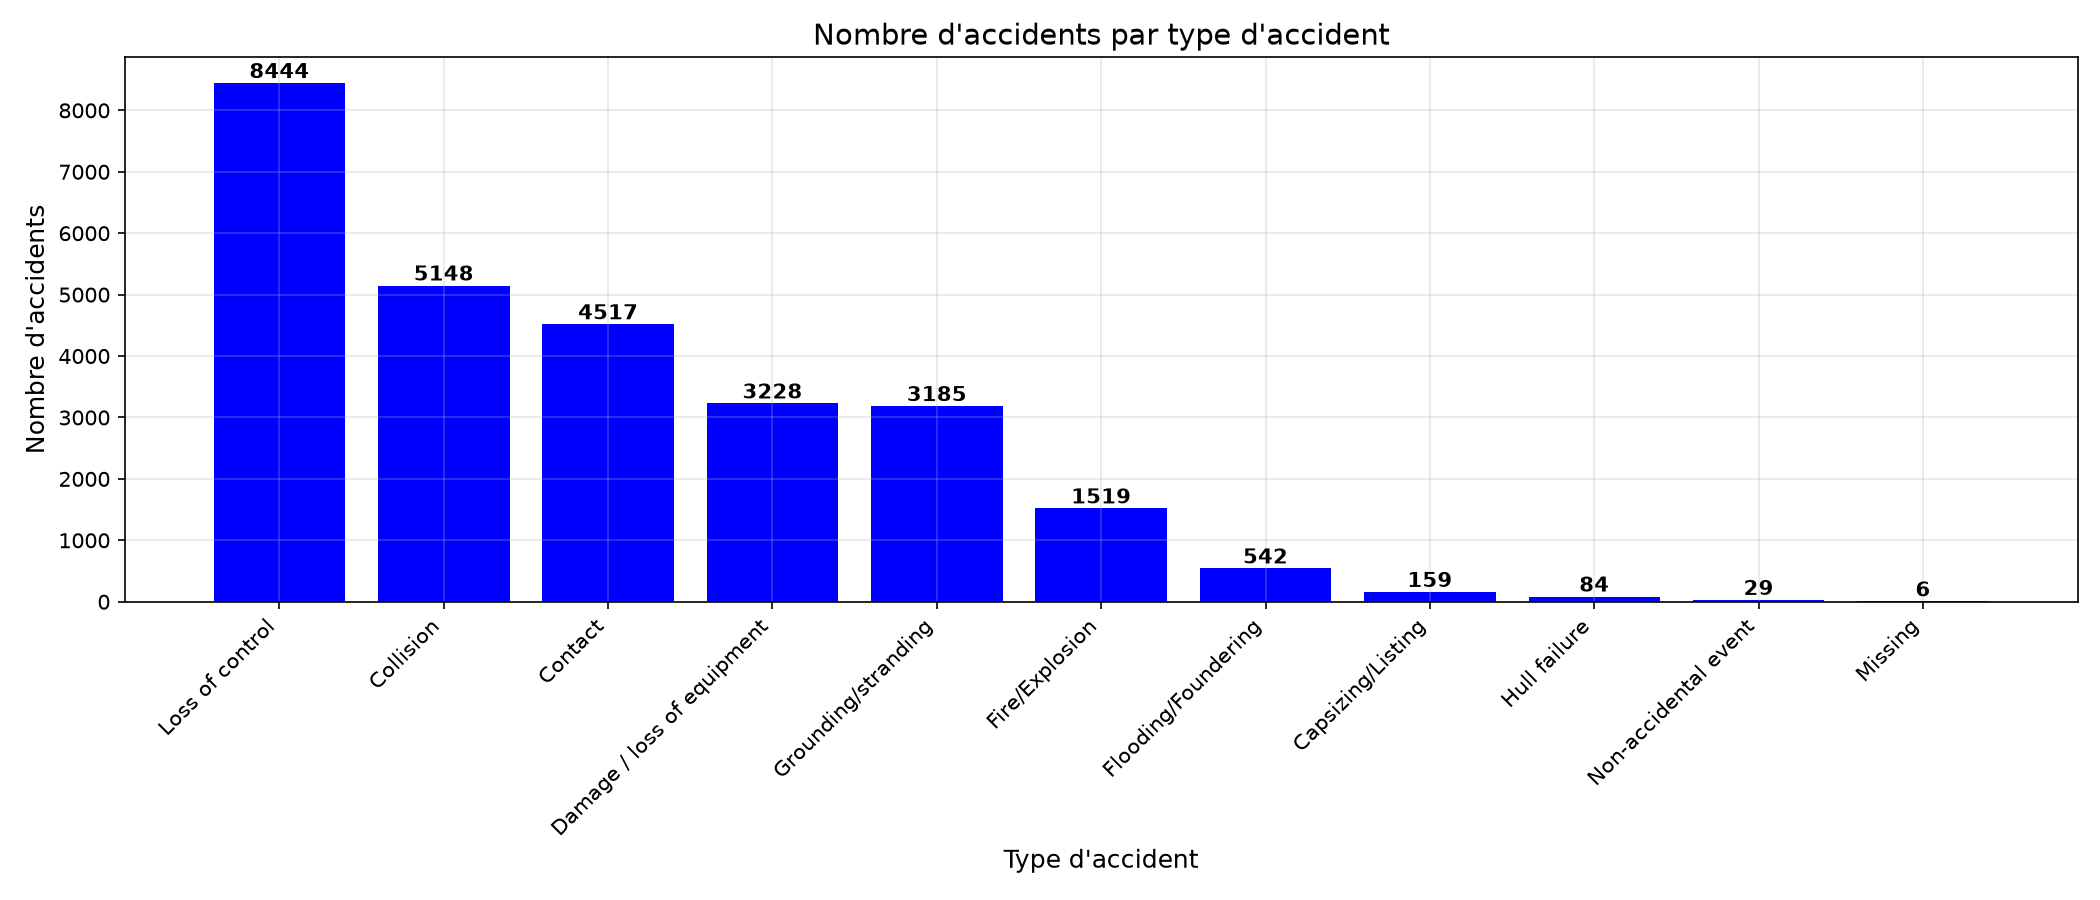
\includegraphics[width=0.9\textwidth]{graph_accident_by_type_europe.png}
  \caption{Répartition des accidents par type.}
  \label{fig:type_accident}
\end{figure}

\textbf{Type d'accident.} La figure~\ref{fig:type_accident} montre la répartition des accidents par type. Trois catégories dominent largement :
\begin{itemize}
  \item \og Loss of control \fg{} : 8~444 cas, perte de contrôle du navire ;
  \item \og Collision \fg{} : 5~148 cas, collision entre navires ($\sim$83,5~\% cause humaine identifiée, le reste événement extérieur tel que la météo) ;
  \item \og Contact \fg{} : 4~517 cas, un accrochage avec un objet fixe ou flottant (autre qu'un navire).
\end{itemize}
Ensuite il y a les dommages ou pertes d'équipement (3~228 cas), les échouements (3~185 cas) et les incendies/explosions (1~519 cas). Les autres types comme par exemple défaillance de coque sont minoritaires. Ces résultats montrent une forte prédominance des pertes de contrôle, des collisions et des contacts parmi les types d'accidents enregistrés.


\begin{figure}[H]
    \centering
    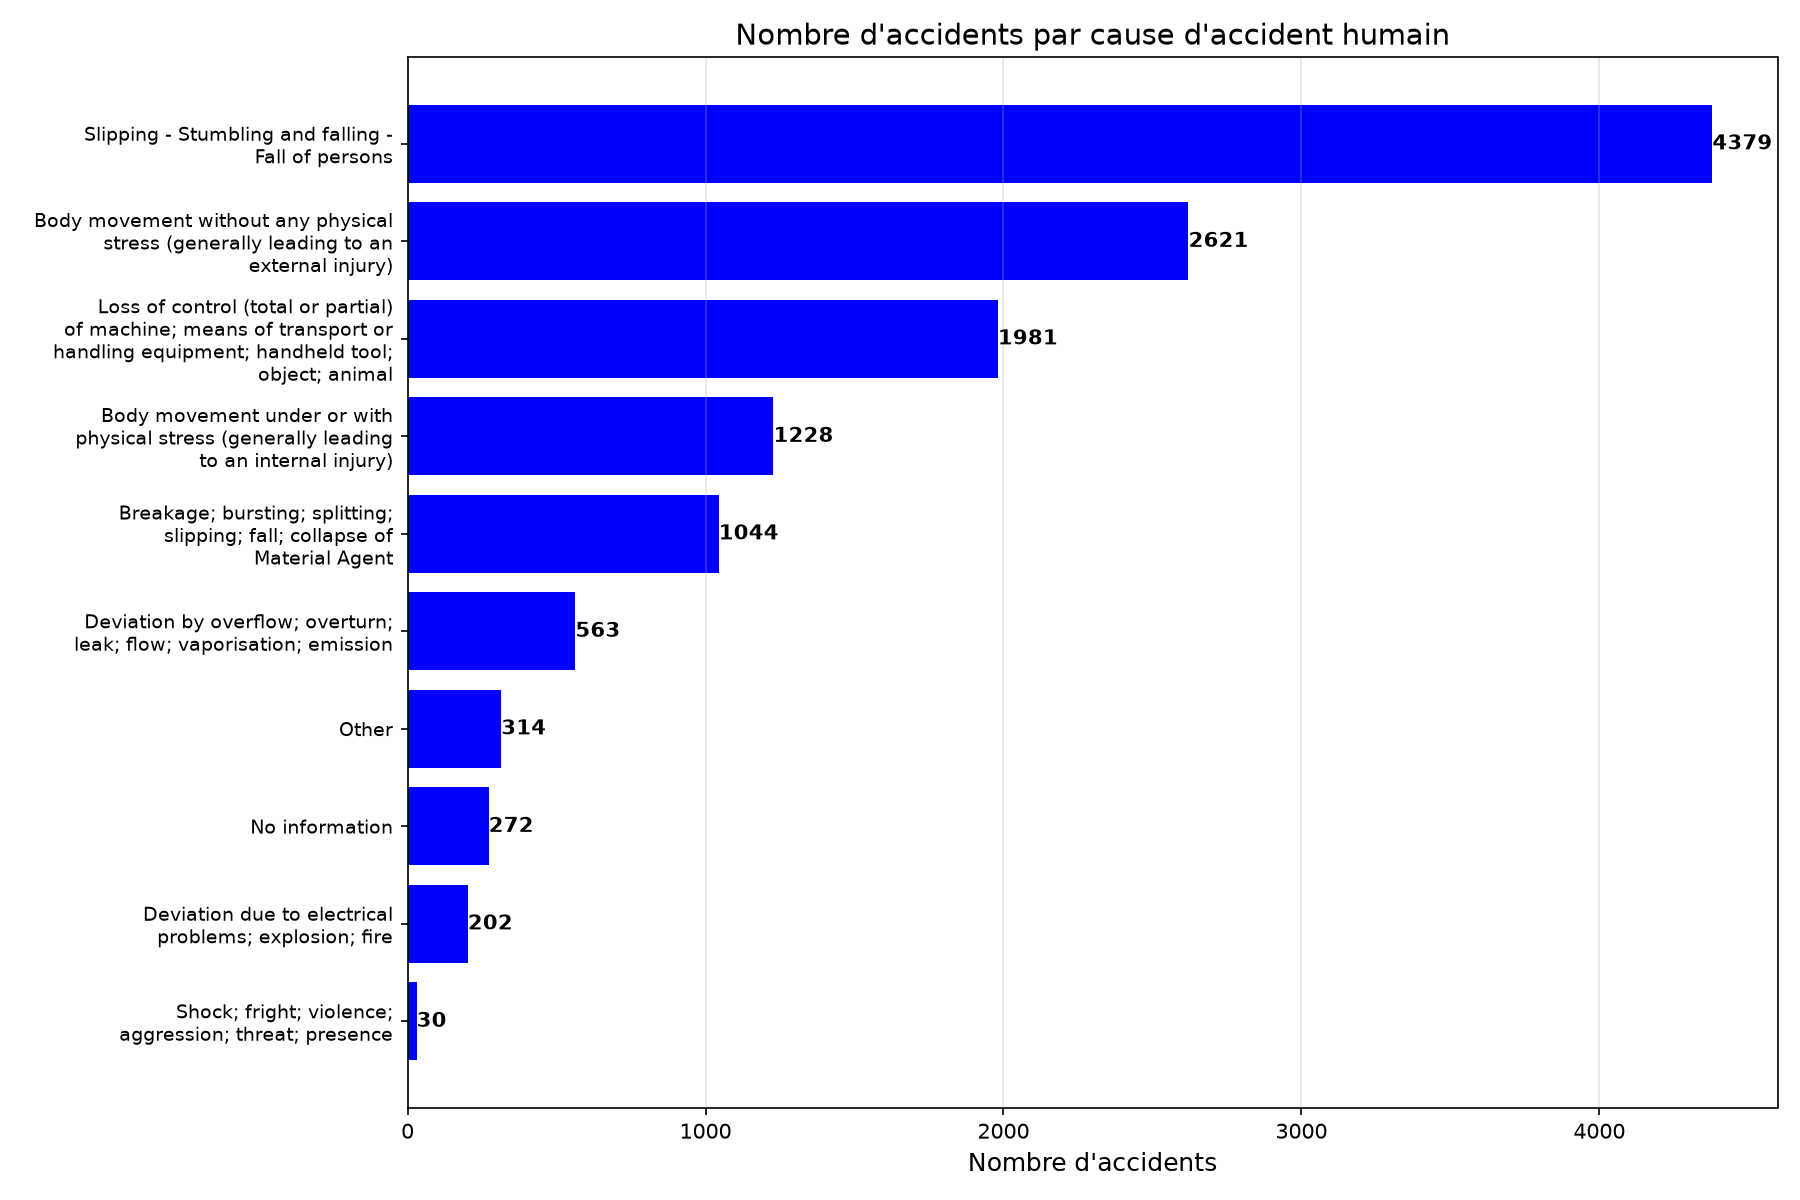
\includegraphics[width=0.9\textwidth]{human_cause_accidents_europe.png}
    \caption{Répartition des causes humaines identifiées dans les accidents.}
    \label{fig:cause_humaine}
\end{figure}
\textbf{Cause humaine.} La figure~\ref{fig:cause_humaine} présente les causes humaines identifiées dans les accidents. On peut constater une prédominance des chutes de personnes (Slipping -- Stumbling -- Falling, 4~379 cas), suivies des mouvements du corps sans contrainte physique (un équipement tombe et blesse quelqu'un ou une vague secoue le navire, une personne se cogne, 2~621 cas) et des pertes de contrôle de machines ou d'équipements (1~981 cas).
Ce qui nous montre que le facteur humain est une cause majeure des accidents. Les chutes et les mouvements inadaptés représentent à eux seuls plus de la moitié des causes connues. On pourrait suggérer que des mesures de prévention ciblant les conditions de travail à bord pourraient potentiellement réduire le nombre d'accidents.



\begin{figure}[H]
  \centering
  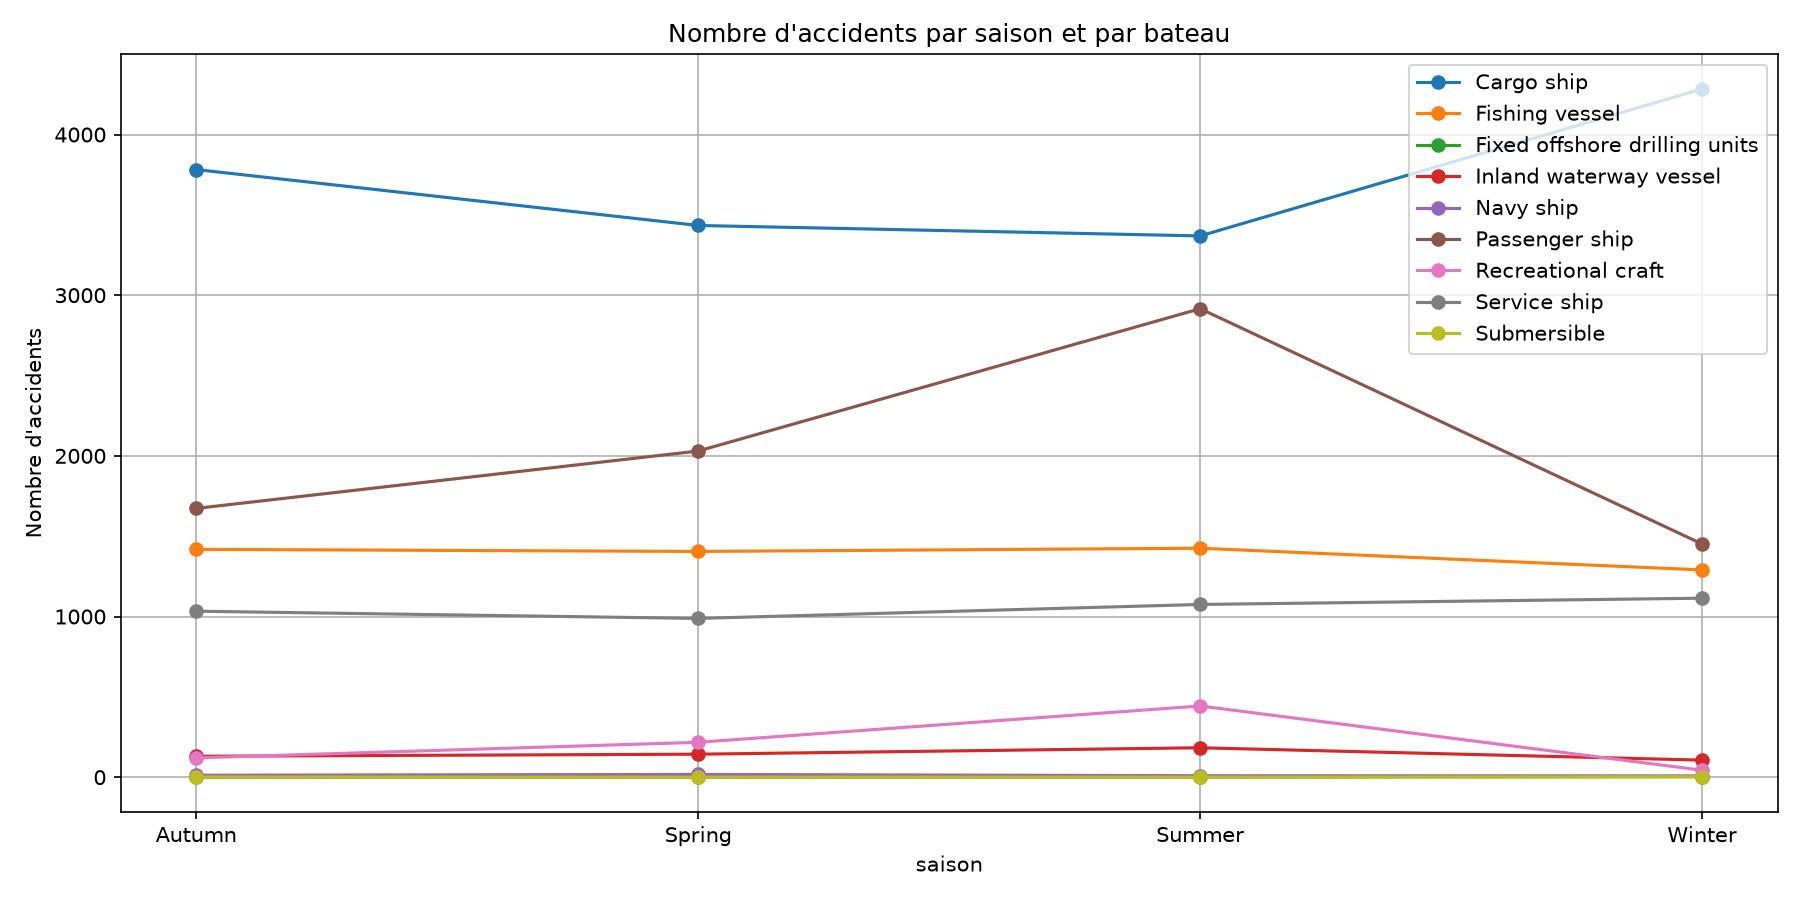
\includegraphics[width=0.9\textwidth]{accidents_by_saison_and_bateau_europe.png}
  \caption{Nombre d'accidents par saison et par type de navire.}
  \label{fig:saison_bateau}
\end{figure}
\textbf{Influence saisonnière et type de navire.} La figure~\ref{fig:saison_bateau} croise le nombre d'accidents par saison et par type de navire. On observe des dynamiques très différentes selon les catégories :

\begin{itemize}
    \item \textbf{Cargos (Cargo ship)} : les plus accidentés toute l'année, avec un pic en hiver ($\sim$4~300 cas) et un minimum en été ($\sim$3~400 cas). Cette évolution peut être mise en relation avec la variation de l'activité de ces navires selon les saisons.
    \item \textbf{Navires à passagers (Passenger ship)} : tendance inverse, avec un maximum en été ($\sim$2~900 cas) et un minimum en hiver ($\sim$1~500 cas). Cette tendance reflète la saisonnalité du tourisme maritime.
    \item \textbf{Navires de pêche (Fishing vessel)} et \textbf{de service (Service ship)} : relativement stables sur l'année, avec des variations faibles ($\sim$1~000 pour la pêche et 1~400 cas pour le service).
    \item \textbf{Autres catégories} (plaisance, sous-marins, offshore) : part beaucoup plus faible des accidents enregistrés.
\end{itemize}

On peut donc conclure que la saisonnalité des accidents dépend fortement du type de navire.

\section{Analyse de la densité du trafic maritime}

La répartition de la densité du trafic maritime présente de nombreux points communs avec celle des accidents étudiée précédemment. Les zones où le trafic est le plus dense correspondent globalement aux zones où l’on observe le plus d’accidents, notamment en mer du Nord, dans la Manche, autour du détroit de Gibraltar, Méditerranée et au niveau du détroit des Dardanelles. Cette observation suggère un lien entre le trafic maritime et la répartition des accidents. La densité du trafic pourra donc être utilisée comme une variable importante dans la suite afin d’analyser son influence sur les accidents et sur l’identification des zones à risque.



% ============================================================
% CHAPITRE 5 : MÉTHODOLOGIE ET MODÉLISATION
% ============================================================
% ============================================================
% CHAPITRE 5 : MÉTHODOLOGIE ET MODÉLISATION
% ============================================================
\chapter{Méthodologie et modélisation}

\section{Approche retenue}

Après l'analyse exploratoire des données, nous avons dans un premier temps testé une régression linéaire afin d'obtenir une première approche de la prédiction du nombre d'accidents. Cependant, cette méthode repose sur une relation linéaire entre les variables et représente donc l'évolution sous la forme d'une droite. Elle est ainsi moins adaptée à nos données, qui présentent des variations et des évolutions ne suivant pas nécessairement une tendance linéaire. Nous avons donc rapidement orienté notre travail vers une Random Forest, permettant de prendre en compte des relations plus complexes entre les différentes variables.

Nous avons étudié cette méthode selon deux approches : une régression, permettant d'estimer le nombre d'accidents, et une classification, permettant d'identifier les tendances d'évolution des accidents dans les différentes cellules de la grille. Pour chaque approche, les années 2023 à 2025 sont utilisées comme données de test afin d'évaluer la fiabilité de nos prédictions.

\section{Random Forest -- Régression}

Le Random Forest en régression nous a permis d'estimer le nombre d'accidents par zone et par année. Un Random Forest est une méthode d'apprentissage automatique qui combine plusieurs arbres de décision afin d'obtenir une prédiction plus fiable. Chaque arbre réalise sa propre prédiction, puis les résultats sont combinés pour obtenir la prédiction finale.

Le modèle utilise plusieurs variables liées à la densité du trafic maritime ainsi qu'une référence historique du nombre d'accidents. Il est composé de 300 arbres, avec une profondeur maximale de 10. Les prédictions sont ensuite agrégées sur notre grille de 1,5° $\times$ 1,5° afin d'obtenir une estimation du nombre d'accidents par zone.

Cependant, la prédiction d'un nombre exact d'accidents reste difficile en raison des nombreuses variations présentes. Nous avons donc choisi de nous orienter vers une approche basée sur la prédiction des tendances, permettant d'identifier plus simplement si une zone est susceptible de connaître une baisse ou une hausse du nombre d'accidents.

\section{Random Forest -- Classification des tendances}

Nous avons ensuite utilisé un Random Forest en classification afin de prédire la tendance d'évolution du nombre d'accidents par zone. Contrairement à la régression, l'objectif n'est plus de prédire un nombre exact, mais de déterminer si le nombre d'accidents est susceptible de diminuer, d'augmenter ou de rester stable.

Nous avons défini 5 classes : forte diminution, faible diminution, stable, faible augmentation et forte augmentation. La classe \og stable \fg{} est de très loin la plus représentée, ce qui risque de conduire le modèle à privilégier cette classe au détriment des autres. Pour pallier ce problème, nous avons cherché à mieux répartir les données entre les différentes tendances.

Pour cela, la classe \og stable \fg{} a été divisée en trois sous-classes : C1, C2 et C3. Cette division permet de répartir la classe majoritaire en plusieurs groupes afin de limiter son influence sur l'apprentissage du modèle. Pour chaque sous-classe, les autres classes sont ensuite comparées afin d'entraîner plusieurs modèles. On fait une moyenne de ces résultats, ce qui permet de déterminer la tendance finale.

Afin d'améliorer les performances du modèle, une validation croisée (\textit{cross validation}) a été mise en place. Le principe consiste à entraîner et évaluer plusieurs fois un modèle sur différentes parties des données, afin de vérifier sa fiabilité et de limiter le risque de dépendre d'un seul découpage des données. Enfin, plusieurs périodes d'agrégation ont été testées : mois, trimestre, semestre et année. Les résultats obtenus avec ces différentes approches sont présentés dans le chapitre suivant.

Pour mieux rééquilibrer les classes, nous avons également choisi de regrouper les tendances en 3 classes principales : Diminution, Stable et Augmentation.

\section{Validation des modèles}

Afin d'évaluer les performances de nos modèles, nous avons comparé les prédictions obtenues avec les données réelles des années 2023, 2024 et 2025. Les modèles sont entraînés à partir de 2013, en raison du manque d'informations avant cette date, jusqu'en 2022. Les prédictions sont ensuite comparées aux tendances réellement observées pour les années suivantes.

Pour la classification des tendances, nous avons utilisé l'\textit{accuracy}, qui correspond au pourcentage de prédictions correctement classées. Elle permet ainsi de mesurer la capacité du modèle à prédire correctement les tendances d'évolution.

\section{Importance des variables}

% ============================================================
% CHAPITRE 6 : RÉSULTATS
% ============================================================
\chapter{Résultats}

\section{Résultats de l'analyse exploratoire}

\section{Performances des modèles}

\section{Carte des prédictions}

\section{Carte des erreurs}

\section{Carte des zones à risque}

\section{Carte des tendances}

\section{Interprétation des résultats}


% ============================================================
% CHAPITRE 7 : CONCLUSION
% ============================================================
\chapter{Conclusion}


% ============================================================
% CHAPITRE 8 : RESSENTI
% ============================================================
\chapter{Ressenti sur le projet tutoré et la licence}


% ============================================================
% BIBLIOGRAPHIE
% ============================================================
\chapter*{Bibliographie}
\addcontentsline{toc}{chapter}{Bibliographie}


% ============================================================
% ANNEXES
% ============================================================
\chapter*{Annexes}
\addcontentsline{toc}{chapter}{Annexes}

\end{document}